\documentclass[12pt, a4paper]{article}

\usepackage[pdftex]{graphicx}

\usepackage{tikz}
\usepackage{rotating}
\usetikzlibrary{patterns}

% Graphs for tikz
% https://github.com/caro811/graphs-tikz

%---------------------------------------------------------------------------------------------------
% Vertices

% \vertex[(optional) color]{x}{y}{name}
\newcommand{\vertex}[4][black]{
    \draw[#1, fill=#1, inner sep=0pt] (#2, #3) circle (0.075) node(#4){};
}

% Vertex (unlabelled) of medium size
% \vertexMedium[optional arguments (for example, color, pattern)]{x}{y}{name}
\newcommand{\vertexMedium}[4][]{
	\path (#2,#3) node[draw, circle, #1, minimum width=15pt](#4){};
}

% With label inside
% \vertexLabelledInside[optional arguments (for example, color, pattern)]{x}{y}{name}{label}
\newcommand{\vertexLabelledInside}[5][]{
	\path (#2,#3) node[draw, circle, #1, minimum width=25pt](#4){#5};
}

% Only label, outside
% \vertexLabel[(optional) position]{name}{label}
% position: below, above, left, right, and combinations (below left, etc.)
\newcommand{\vertexLabel}[3][above]{
    \path (#2) node[#1]{#3};
}
%---------------------------------------------------------------------------------------------------

%---------------------------------------------------------------------------------------------------
% Edges

% Straight
% \edge[optional parameters (such as "color=red, dashed")]{nameVertex1}{nameVertex2}
\newcommand{\edge}[3][]{
	\draw[#1] (#2) -- (#3);
}

% Curved
% \edgeCurved[optional parameters (such as "color=red, dashed")]{nameVertex1}{nameVertex2}{angleOut}{angleIn}
\newcommand{\edgeCurved}[5][]{
	\draw[#1] (#2) to[out=#4, in=#5] (#3);
}

% Only label
% \edgeLabel[(optional) position]{nameVertex1}{nameVertex2}{label}
\newcommand{\edgeLabel}[4][above]{
	\path (#2) -- (#3) node[midway, #1]{#4};
}
%---------------------------------------------------------------------------------------------------

%---------------------------------------------------------------------------------------------------
% Join
% \join[optional parameters (such as "color=red, dashed")]{name graph 1}{n1}{name graph 2}{n2}
\newcommand{\join}[5][]{
	\foreach \joinI in {1,...,#3} {
		\foreach \joinJ in {1,...,#5} {
			\edge[#1]{#2\joinI}{#4\joinJ};
		}
	}
}
%---------------------------------------------------------------------------------------------------

%---------------------------------------------------------------------------------------------------
% Vertex of a regular polygon
% \vertexRegularPolygon[(optional) color]{x of center}{y of center}{scale}{n}{position of vertex}{name}
\newcommand{\vertexRegularPolygon}[7][]{
	\vertex[#1]
	{ { (#2) + (#4) * -cos(deg(6.283*(#6 - 1)/(#5)-(1.571+3.142/(#5)))) } }
	{ { (#3) + (#4) * sin(deg(6.283*(#6 - 1)/(#5)-(1.571+3.142/(#5)))) } }
	{#7};
}
%---------------------------------------------------------------------------------------------------

%---------------------------------------------------------------------------------------------------
% Cycle
% \cycle[(optional) color]{x of center}{y of center}{scale}{n}{name}
\newcommand{\cycle}[6][]{
	\foreach \cycleI in {1,...,#5} {
		\vertexRegularPolygon[#1]
						{#2}{#3}
						{#4}
						{#5}
						{\cycleI}
						{#6\cycleI}
						{};
	}

	\foreach \cycleI in {2,...,#5} {
		\pgfmathtruncatemacro{\cycleIminusOne}{\cycleI - 1};

		\edge[#1]{#6\cycleI}{#6\cycleIminusOne};
	}
	\pgfmathtruncatemacro{\cycleN}{#5};
	\pgfmathtruncatemacro{\cycleOne}{1};
	\edge[#1]{#6\cycleN}{#6\cycleOne};
}
%---------------------------------------------------------------------------------------------------

%---------------------------------------------------------------------------------------------------
% Complete
% \complete[(optional) color]{x of center}{y of center}{scale}{n}{name}
\newcommand{\complete}[6][]{
	\foreach \completeI in {1,...,#5} {
		\vertexRegularPolygon[#1]
						{#2}{#3}
						{#4}
						{#5}
						{\completeI}
						{#6\completeI}
						{};
	}

	\foreach \completeI in {2,...,#5} {
		\pgfmathtruncatemacro{\completeIminusOne}{\completeI - 1};

		\foreach \completeJ in {1,...,\completeIminusOne} {
			\edge[#1]{#6\completeI}{#6\completeJ};
		}
	}
}
%---------------------------------------------------------------------------------------------------

%---------------------------------------------------------------------------------------------------
% Spiders with no head (H = \emptyset)

% Thin spider
% \thinSpider[(optional) color]{x of center}{y of center}{scale}{n}{name}
\newcommand{\thinSpider}[6][]{
	\foreach \thinSpiderI in {1,...,#5} {
		\vertexRegularPolygon[#1]
						{#2}{#3}
						{#4}
						{#5}
						{\thinSpiderI}
						{#6c\thinSpiderI}
						{};

		\vertexRegularPolygon[#1]
						{#2}{#3}
						{2*(#4)}
						{#5}
						{\thinSpiderI}
						{#6s\thinSpiderI}
						{};

		\edge[#1]{#6c\thinSpiderI}{#6s\thinSpiderI};
	}

	\foreach \thinSpiderI in {2,...,#5} {
		\pgfmathtruncatemacro{\thinSpiderIminusOne}{\thinSpiderI - 1};

		\foreach \thinSpiderJ in {1,...,\thinSpiderIminusOne} {
			\edge[#1]{#6c\thinSpiderI}{#6c\thinSpiderJ};
		}
	}
}

% Fat spider
% \fatSpider[(optional) color]{x of center}{y of center}{scale}{n}{name}
\newcommand{\fatSpider}[6][]{
	\foreach \fatSpiderI in {1,...,#5} {
		\vertexRegularPolygon[#1]
						{#2}{#3}
						{#4}
						{#5}
						{\fatSpiderI}
						{#6c\fatSpiderI}
						{};

		\vertexRegularPolygon[#1]
						{#2}{#3}
						{2*(#4)}
						{#5}
						{\fatSpiderI}
						{#6s\fatSpiderI}
						{};
	}

	\foreach \fatSpiderI in {2,...,#5} {
		\pgfmathtruncatemacro{\fatSpiderIminusOne}{\fatSpiderI - 1};

		\foreach \fatSpiderJ in {1,...,\fatSpiderIminusOne} {
			\edge[#1]{#6c\fatSpiderI}{#6c\fatSpiderJ};
		}
	}

	\foreach \fatSpiderI in {1,...,#5} {
		\foreach \fatSpiderJ in {1,...,#5} {
			\ifthenelse
			{\equal{\fatSpiderI}{\fatSpiderJ}}
			{}
			{\edge[#1]{#6s\fatSpiderI}{#6c\fatSpiderJ};};
		}
	}
}
%---------------------------------------------------------------------------------------------------


%------------------------------------------------------------------------------------------------------------------------------------
%------------------------------------------------------------------------------------------------------------------------------------
\begin{document}

Graphs for tikz. Examples.

\bigskip

\begin{center}
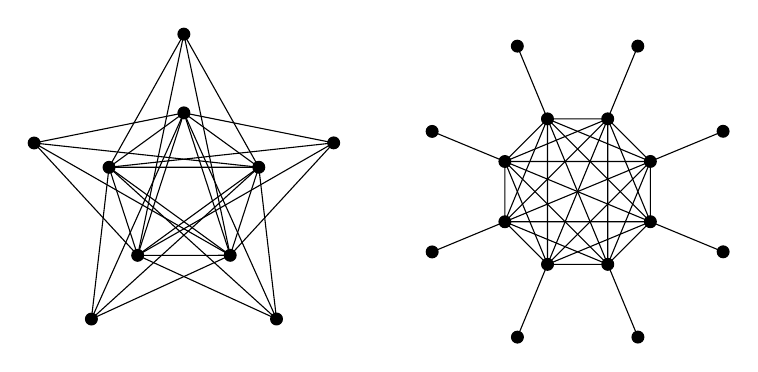
\begin{tikzpicture}
	\fatSpider{0}{0}{1}{5}{f};

	\thinSpider{5}{0}{1}{8}{f};
\end{tikzpicture}
\end{center}

\bigskip

\begin{center}
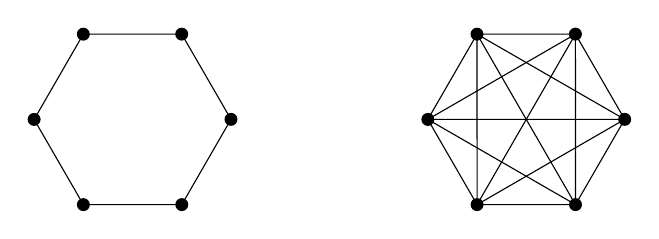
\begin{tikzpicture}
	\cycle{0}{0}{1.25}{6}{c};

	\complete{5}{0}{1.25}{6}{k};
\end{tikzpicture}
\end{center}

\bigskip

\begin{center}

\begin{tikzpicture}
	\vertex[green]{0}{0}{v};

	\vertexLabel{v}{N};
	\vertexLabel[green, above right]{v}{NE};
	\vertexLabel[right]{v}{E};
	\vertexLabel[green, below right]{v}{SE};
	\vertexLabel[below]{v}{S};
	\vertexLabel[green, below left]{v}{SO};
	\vertexLabel[left]{v}{O};
	\vertexLabel[green, above left]{v}{NO};
\end{tikzpicture}
\hspace{50pt}
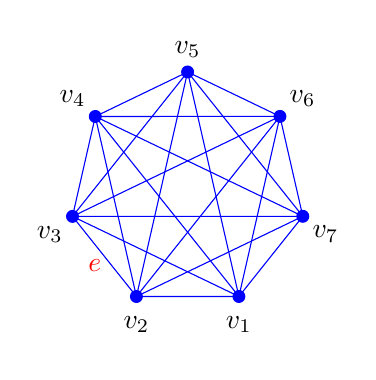
\begin{tikzpicture}
	\complete[blue]{0}{0}{1.5}{7}{K};

	\vertexLabel[below, inner sep=7pt]{K1}{$v_1$};
	\vertexLabel[below, inner sep=7pt]{K2}{$v_2$};
	\vertexLabel[below left]{K3}{$v_3$};
	\vertexLabel[above left]{K4}{$v_4$};
	\vertexLabel[above, inner sep=5pt]{K5}{$v_5$};
	\vertexLabel[above right]{K6}{$v_6$};
	\vertexLabel[below right]{K7}{$v_7$};

	\edgeLabel[red, below left, inner sep=1pt]{K2}{K3}{$e$};
\end{tikzpicture}
\end{center}

\bigskip

\begin{center}
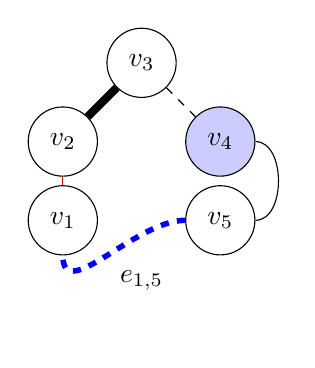
\begin{tikzpicture}
	\vertexLabelledInside{0}{0.75}{v1}{$v_1$};
	\vertexLabelledInside{0}{1.75}{v2}{$v_2$};
	\vertexLabelledInside{1}{2.75}{v3}{$v_3$};
	\vertexLabelledInside[fill=blue!20]{2}{1.75}{v4}{$v_4$};
	\vertexLabelledInside{2}{0.75}{v5}{$v_5$};

	\edge[color=red]{v1}{v2};
	\edge[line width=3pt]{v2}{v3};
	\edge[dashed]{v3}{v4};
	\edgeCurved{v4}{v5}{0}{0};
	\edgeCurved[dashed, color=blue, line width=2pt]{v5}{v1}{180}{270};
	\edgeLabel[below, inner sep=18pt]{v5}{v1}{$e_{1,5}$};
\end{tikzpicture}
\hspace{50pt}
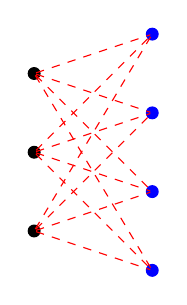
\begin{tikzpicture}
	\vertex{0}{0.5}{a1};
	\vertex{0}{1.5}{a2};
	\vertex{0}{2.5}{a3};
	\vertex[blue]{1.5}{0}{b1};
	\vertex[blue]{1.5}{1}{b2};
	\vertex[blue]{1.5}{2}{b3};
	\vertex[blue]{1.5}{3}{b4};

	\join[red, dashed]{a}{3}{b}{4};
\end{tikzpicture}
\hspace{50pt}
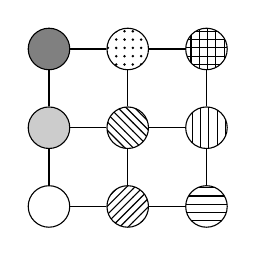
\begin{tikzpicture}
	\vertexMedium{0}{0}{g00};
	\vertexMedium[fill=black!20]{0}{1}{g01};
	\vertexMedium[fill=gray]{0}{2}{g02};
	\vertexMedium[pattern=north east lines, pattern color=black]{1}{0}{g10};
	\vertexMedium[pattern=north west lines, pattern color=black]{1}{1}{g11};
	\vertexMedium[pattern=dots, pattern color=black]{1}{2}{g12};
	\vertexMedium[pattern=horizontal lines, pattern color=black]{2}{0}{g20};
	\vertexMedium[pattern=vertical lines, pattern color=black]{2}{1}{g21};
	\vertexMedium[pattern=grid, pattern color=black]{2}{2}{g22};

	\edge{g00}{g01};
	\edge{g00}{g10};
	\edge{g01}{g02};
	\edge{g01}{g11};
	\edge{g02}{g12};
	\edge{g10}{g11};
	\edge{g10}{g20};
	\edge{g11}{g12};
	\edge{g11}{g21};
	\edge{g12}{g22};
	\edge{g20}{g21};
	\edge{g21}{g22};
\end{tikzpicture}
\end{center}
%-------------------
\end{document}
